\section{Introduction}

[In the previous chapter (DMFs) I show the evolution in dust masses assuming Galactic dust at all redshifts (i.e T=20K and beta=2), this chapter will tackle this assumption.]

\section{Dust Properties of DSFGs}

Interstellar dust plays a crucial role in the formation of galaxies as dust grains are the site of molecule formation like molecular hydrogen, $H_2$, the primary fuel for star formation (\citealt{Kennicutt_2012}). $H_2$ is the most abundant molecule in the Universe but is difficult to observe directly unless originating from energetic environments. Alternatives include observing less abundant molecules such as CO and using conversion factors to estimate the mass of molecular hydrogen, or observing dust emission to estimate dust masses (as in the previous chapter) and assuming gas-to-dust ratios (e.g. \citealt{Saintonge_2013}) to convert these into estimates for the total gas mass in high-redshift galaxies (e.g. \citealt{Magdis_2012}; \citealt{Eales_2012}; \citealt{Scoville_2014}; \citealt{Santini_2014}; \citealt{Genzel_2015}). Such studies have shown that galaxies at high redshift contain a higher fraction of gas than galaxies today (\citealt{Tacconi_2010}; \citealt{Scoville_2016}; \citealt{Scoville_2017}; \citealt{Millard_2020}), showing that direct observations of dust emission are useful in our understanding of how galaxies grow and evolve. It is important to note, however, that studies that make these links between dust emission and the evolution of galactic properties make the basic assumption that properties of the dust remain constant with redshift. In the following we investigate the possibility of evolution in dust itself by modelling the dust emission from a sample of high-redshift galaxies and measuring their dust properties over a large expanse of cosmic history.

Of particular importance to us is the dust emissivity spectral index, $\beta$, which controls the frequency dependence of the emissivity of dust grains per unit mass. By assuming, as is customary, that the optical depth of a galaxy can be approximated as a power law of the form $\tau \propto \nu^\beta$, we are implicity assuming that $\beta$ encodes within it information about the dust grain properties such as their chemical composition and their size and growth. The assumed value of $\beta$ for a galaxy can have significant consequences on the assumed absorption properties of the dust grains and consequently on fundamental properties of the ISM in the galaxy such as the total mass of dust (\citealt{Bianchi_2013}; \citealt{Clark_2016}).

Theoretical models for dust (e.g. \citealt{Draine_1984}; \citealt{Draine_2011}; \citealt{Kohler_2015}) predict $\beta$ values to range between approximately 1 -- 2 depending on the chemical composition of the dust grains. Adopting suitable fixed values of $\beta$ have been vital for estimates of the dust temperature and dust luminosity of galaxies in past studies, particularly for high-redshift sources that often lack constraints in the far-infrared (e.g. \todo[color=green]{Add references}). A nominal value of $\beta$ = 2 is common practice in this scenario as it mimics the emissivity of mixtures of amorphous silicates and graphites that well represent the optical properties of Galactic dust grains. However, recent studies have shown that the value of $\beta$ can take a wide variety of values among local galaxies and even among different regions within the same galaxy. For example, \citealt{Lamperti_2019} model the far-infrared dust SEDs of 192 nearby galaxies from the JCMT dust and gas In Nearby Galaxies Legacy Exploration (JINGLE) survey and observed a range of temperatures for the cold dust between 17 and 30\,K and dust emissivity spectral indices between 0.6 and 2.2. Within M31 (Andromeda) \citealt{Smith_2012}, \citealt{Draine_2014} and \citealt{Whitworth_2019} identified a decrease in $\beta$ with galactocentric radius, potentially a result of $\beta$ evolving to higher values when observed in denser regions of the ISM due to grain coagulation. A follow up study by \citealt{Athikkat-Eknath_2022} compared the average $\beta$ measured inside and outside molecular clouds within M31, and while there was no evidence to support the idea that $\beta$ varies due to dense molecular gas, the radial variation in $\beta$ remained present. At higher redshifts, where the far-infrared part of the spectrum is spatially unresolved, it is not possible to constrain the true value of a galaxy's $\beta$ but can be used to define an \textit{effective} $\beta$ value that represents the integrated dust properties over the whole galaxy. [...]\todo[color=orange]{Importance of having an effective $\beta$ value.}

\section{Obtaining Redshifts from Carbon Monoxide Lines}

In order to study the evolution of the dust properties of DSFGs we require robust redshifts to place their formation in cosmic history and to determine accurate measurements of fundamental properties. Obtaining robust ages of galaxies in the form of spectroscopically determined redshifts is hampered by the poor spatial resolution of single-dish observations, which worsens with increasing redshift. While DSFGs can be discovered at far-infrared and sub-mm wavelengths to high redshifts directly from the photometry of the sub-mm source, selecting those with distinctly red sub-mm colours in the \textit{Herschel} bands (e.g. \citealt{Dowell_2014}; \citealt{Ivison_2016}; \citealt{Donevski_2018}; \citealt{Duivenvoorden_2018}), careful consideration of the selection wavelength is required to make optimal use of the negative K-correction. For example, the \textit{Herschel}-SPIRE bands increasingly probe the peak of the dust SED at higher redshifts, making them less sensitive to unlensed DSFGs beyond z $\sim$ 2 -- 3. Additionally, the dust-obscured nature of this population of galaxies makes the identification of counterparts at other wavelengths where spectroscopically determined reshifts are readily available more difficult, which is compounded by the poor resolution and source confusion in the sub-mm (see the Likelihood Ratio analysis of Chapter \ref{chapter:Data_Release_3} for an example).

A more reliable method for robust redshifts is to follow up single-dish observations with inteferometric measurements with interferometers such as the Atacama Large Millimeter/submillimeter Array (ALMA). An even more direct way of obtaining redshfits while observing sources in the sub-mm/mm wavebands is to observe molecular emission lines which can be directly associated with the sub-mm emission without the need for intermediary steps with high-resolution imaging. Recent advancements in the possible bandwidths of instruments like ALMA and the Northern Extended Millimetre Array (NOEMA) have allowed for the ability to detect spectral lines (typically from CO or [CII]) that emanate unambiguously from the sub-mm source. CO is the second most abundant molecule in the Universe after $H_2$ and has rotational transitions that produce some of the brightest lines in the millimeter spectrum. The brightness of the CO lines result from the abundance of CO, the low excitation energy of the transitions and the wavelengths at which they occur coinciding with regions of the spectrum with high atmospheric transmission probed by ALMA. A secondary advantage of using molecular emission to determine spectroscopic redshifts is that they are independent of the photometry used to describe the dust SED and are therefore less prone to bias. In Figure \ref{fig:redshift_ladder} I show the coverage of CO line transitions as functions of the redshift and observed wavelength. We see that at [...] wavelengths, there is a non-uniform coverage of CO transitions, meaning that sources believed to be at a particular redshift may have multiple line detections, allowing for unambiguous constraints on the redshift of the galaxy, single line detections, which allows for some abiguity to the redshift solution, or no line detections. In the regions where no CO lines can be detected by a particular instrument, "redshift deserts" appear as breaks in the redshift distribution of galaxies.

\begin{figure}
	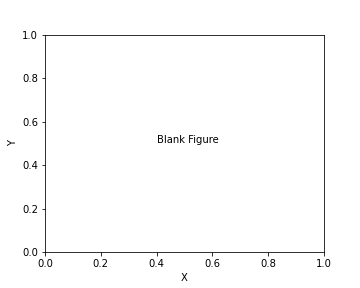
\includegraphics[width=\columnwidth]{Figures/blank_figure.png}
	\caption{Caption}
	\label{fig:redshift_ladder}
\end{figure}

In this work I study bright infrared sources detected by \textit{Herschel} and the South Pole Telescope (SPT; \citealt{Carlstrom_2011}) that have spectroscopically determined redshifts to test whether their measured dust properties have evolved from the early Universe to the peak epoch of star formation (between 2 $\lesssim z_{\textrm{spec}} \lesssim$ 6). We are also interested in identifying possible diversity in the dust properties of DSFGs and whether differing selection methods influence the type of dust that is observed. I therefore implicity assume in the following work that changes in the properties of the interstellar dust in galaxies can be directly inferred from variations in the spectral index, $\beta$ and the temperature of dust grains.

\section{Sample Creation}
\subsection{South Pole Telescope DSFGs}

A population of IR-bright SMGs selected at 1.4\,mm were obtained from the South Pole Telescope - Sunyarv-Zel'dovich (SPT-SZ) survey (\citealt{Everett_2020}) which covers approximately 2500\,deg$^2$. The depth of this survey reaches $\sim$ 20\,mJy at 1.4\,mm, corresponding to sources detected at greater than 4.5\,$\sigma$ significance. I define our SPT sample as the 81 sources that have had synchrotron dominated systems removed (based on their 1.4\,mm to 2\,mm flux density ratios) and flux-limited to $S_{\textrm{870\,\micron}}$ > 25\,mJy. The high flux density cuts imply that most IR-bright galaxies would be too faint for the SPT sample without having been magnified from gravitational lensing. As shown by \citealt{Weiss_2013}, the average magnification of these sources are $\mu \sim$ 15 (corresponding to intrinsic flux densities of $S_{1.4\,\textrm{mm}}$ = 1 -- 3\,mJy), which is similar to the flux densities of unlensed sources identified from blank field surveys in the sub-mm/mm wavebands (e.g. \citealt{Coppin_2006}; \citealt{Pope_2006}; \citealt{Weiss_2009}) and are thus likely to be representative of this population albeit at higher observed redshifts.

During ALMA Cycle 0 \citealt{Weiss_2013} conducted a blind redshift survey for 26 SPT sources with ALMA's Band 3 receiver (2.6 -- 3.6\,mm). In total 44 line features were identified in the survey as emission lines of $^{12}$CO, $^{13}$CO, CI, H$_2$O and H$_2$O$^+$. The spectra of the 26 sources could be categorized according to the ambiguity of their estimated redshifts: 12 sources had spectra with multiple clear line features, from which a unique redshift solution can be found from the ALMA scans alone; 11 had a single line feature for which other spectroscopic or photometric measurements would be requied to constrain the redshift; and three sources for which no line features were observed. The same observing strategy was used during ALMA Cycle 1 by \citealt{Strandet_2016} to extend the redshift survey of \citealt{Weiss_2013} with an additional 15 sources observed in ALMA Band 3. For sources with a single CO line detection during Cycle 0, \citealt{Strandet_2016} present ALMA 1\,mm (Band 6) follow-up observations and, when still not satisfactory, follow-up observations were made with the First Light APEX Submillimetre Heterodyne receiver (FLASH; \citealt{Heyminck_2006}), the Swedish-ESO PI receiver (SEPIA; \citealt{Billade_2012}) and the Z-spec camera (\citealt{Naylor_2003}) onboard the Atacama Pathfinder Experiment (APEX) targeting CO and [CII] lines for those that remained unambiguous during Cycles 0 and 1. Lastly, \citealt{Reuter_2020} concluded the SPT redshift survey during ALMA Cycles 3, 4 and 7 by presenting spectra for the remaining 40 of the total 81 sources that had yet to be scanned. This resulted in 41 new spectroscopic redshifts. The culmination of these studies is a sample of 81 SPT-selected DSFGs  each with a spectroscopic redshift in the range 1.9 < $z_{\textrm{spec}}$ < 6.9; the median redshift of the sample being $z_{\textrm{median}}$ = 3.9$\pm$0.2 (\citealt{Reuter_2020}).

\subsection{The HerBS Sample}
\section{Far-Infrared and Sub-mm Colours}
\section{The Modified Blackbody Model}
\section{SED Fitting of DSFGs}
\subsection{Posterior Distributions}
\subsection{The Dust Emissivity Spectral Index - Dust Temperature Degeneracy}
\section{Accuracy of Dust Parameters}
\subsection{Simulations of SPT and HerBS Sources}
\subsection{Results of Simulations}
\section{The Properties of Dust in DSFGs}
\subsection{The Diversity of Dust Emissivity Spectral Indices and their Evolution with Redshift}
\subsection{The Diversity of Dust Temperatures and their Evolution with Redshift}
\subsection{Implications of Evolving Dust Properties between 2 < z < 6}
\section{Conclusions}

\listoftodos